In diesem Themenblock wird das generative Übersetzungsmodell entwickelt, trainiert und evaluiert. Aufbauend auf dem bereinigten Parallelkorpus (Themenblock~1) und der gelernten Komplexitätsmetrik (Themenblock~2) erfolgt die Modellierung über ein zweistufiges Trainingsverfahren: ein überwachtes Feintuning (Supervised Fine-Tuning, SFT) gefolgt von einer direkten Präferenzoptimierung (Direct Preference Optimization, DPO).

\subsection{Supervised Fine-Tuning (SFT)}
\label{sec:sft_training}
\label{sec:daten_splits_dpo}

\subsubsection{Datenbasis, Trainings-Splits \& Sequence-to-Sequence-Modellierung}
\label{sec:sft_korpus_filterung}
\label{sec:split_konfiguration_anti_contamination}
\label{sec:sft_seq2seq}

Als Datenbasis für das überwachte Feintuning (Supervised Fine-Tuning, SFT) dient der bereinigte und qualitätsgesicherte Master-Korpus ($N = 860$ Paare, 11 Webquellen, Themenblock~1). Die maximale Sequenzlänge wird einheitlich auf $L_{\max} = 1.024$ Tokens festgelegt. Für das Modelltraining wird der Datenbestand auf Artikelebene in ein Trainings-Set ($85\,\%$, $N = 680$ Paare) zur Parameteroptimierung sowie ein Validierungs-Set ($15\,\%$, $N = 121$ Paare) für Loss-Tracking und Early Stopping ($\text{Patience} = 10$) aufgeteilt. Wie auch schon bei den Metrikmodellen (Themenblock~2) werden alle generativen Modelle auf dem unabhängigen Out-of-Domain-Datensatz der \textit{Lebenshilfe Schleswig-Holstein e.\,V.} ($N = 37$ Artikelpaare) evaluiert, um eine kontaminationsfreie Bewertung auf professionell erstellter Leichter Sprache zu gewährleisten.

Die Übersetzung von behördlichen und journalistischen Texten in Leichte Sprache wird als monolinguales Text-zu-Text-Transformationsproblem modelliert. Als Basisarchitektur dient das Sequenz-zu-Sequenz-Modell \texttt{facebook/mbart-large-50} \citep{tang2020multilingual, liu2020multilingual}. Die Wahl dieser Architektur stützt sich auf drei Faktoren:
\begin{itemize}
    \item \textbf{Entkopplung von Enkodierung und Generierung:} Der bidirektionale Encoder verarbeitet den gesamten alltagssprachlichen Quelltext simultan über alle Schichten hinweg und erzeugt eine kontextuelle Repräsentation des Inhalts. Der autoregressive Decoder greift über Cross-Attention-Mechanismen gezielt auf diese Repräsentation zu, wodurch eine strikte inhaltliche Quellbindung gewährleistet wird.
    \item \textbf{Multilinguale Voroptimierung \& Denoising-Pretraining:} mBART-50 verfügt über $611\,\text{M}$ Parameter ($12$ Encoder- und $12$ Decoder-Layer, $d_{\text{model}} = 1.024$, $16$ Attention Heads) und wurde auf multilingualen Korpora über Textinfillings und Permutationsaufgaben vortrainiert, was eine hohe Robustheit gegenüber syntaktischen Satzumstellungen verleiht.
    \item \textbf{Zwingende Sprachcode-Initialisierung (\texttt{de\_DE}):} Da mBART-50 über $50$ Sprachen abdeckt, ist die explizite Vorkonfiguration der Sprach-Tokens im Tokenizer und Modell (\code{tokenizer.src_lang = "de_DE"} und \code{tokenizer.tgt_lang = "de_DE"}) unerlässlich. Wird diese Initialisierung unterlassen, neigt das Modell zu Sprachdrift oder generiert fremdsprachige Satzfragmente.
\end{itemize}

Den zweistufigen Gesamtablauf aus überwachtem Feintuning (SFT) und direkter Präferenzoptimierung (DPO) unter Einbindung des gelernten neuronalen Metrikmodells veranschaulicht Abbildung~\ref{fig:sft_dpo_pipeline_overview}.

\begin{figure}[htbp]
\centering
\adjustbox{max width=\textwidth}{%
\begin{tikzpicture}[
    font=\small,
    >=latex,
    thick,
    stepbox/.style={draw=none, fill=none, font=\large\bfseries, align=center},
    modelnode/.style={circle, draw=blue!80!black, fill=blue!15, thick, inner sep=2pt, minimum size=1.25cm, font=\large\bfseries, align=center},
    modelnodealigned/.style={circle, draw=teal!80!black, fill=teal!18, thick, inner sep=2pt, minimum size=1.25cm, font=\large\bfseries, align=center},
    basenode/.style={rectangle, draw=blue!85!black, fill=blue!85!black, text=white, font=\bfseries\small, rounded corners=4pt, inner sep=5pt, align=center},
    processsft/.style={rectangle, draw=orange!90!black, fill=orange!85!black, text=white, font=\bfseries\small, rounded corners=5pt, inner sep=6pt, align=center},
    processdpo/.style={rectangle, draw=teal!90!black, fill=teal!80!black, text=white, font=\bfseries\small, rounded corners=5pt, inner sep=7pt, align=center},
    datanode/.style={rectangle, draw=orange!80!black, fill=orange!12, thick, rounded corners=4pt, inner sep=4pt, align=center},
    promptnode/.style={rectangle, draw=gray!75!black, fill=gray!12, thick, rounded corners=4pt, inner sep=4pt, align=center},
    metricnode/.style={rectangle, draw=purple!80!black, fill=purple!10, thick, rounded corners=5pt, inner sep=5pt, align=center},
    prefdatanode/.style={rectangle, draw=green!60!black, fill=green!12, thick, rounded corners=4pt, inner sep=4pt, align=center},
    flowarrow/.style={->, thick, line width=1.1pt, draw=black!85},
    refarrow/.style={->, dashed, line width=1.0pt, draw=blue!80!black}
]
% Obere Datenebene
\node[datanode] (sft_data) at (5.0, 2.2) {\textbf{Parallelkorpus}\\$(x^{(i)}, y^{(i)})$ ($N = 860$)};
\node[promptnode] (prompts) at (9.6, 2.2) {\textbf{Quelltexte $x$}\\\footnotesize(10kGNAD)};
\node[metricnode, above=0.8cm of prompts] (metric) {\textbf{Metrikmodell}\\\footnotesize$R_{\text{style}} + R_{\text{sem}}$\\\scriptsize\textcolor{purple!90!black}{[Ersetzt Human]}};
\node[prefdatanode, right=1.6cm of metric] (pref_data) {\textbf{Präferenzdaten $\mathcal{D}_{\text{DPO}}$}\\$(x^{(i)}, y_w^{(i)}, y_l^{(i)})$ ($N = 9.246$)};
% Untere Modellebene
\node[basenode] (pretrain) at (0.0, 0) {\textbf{mBART-50}\\\footnotesize Basismodell};
\node[modelnode] (base_pi) at (2.5, 0) {$\boldsymbol{\pi_0}$};
\node[below=0.12cm of base_pi, font=\footnotesize, align=center, text=black!80] {Basismodell};
\node[processsft] (sft_box) at (5.0, 0) {\textbf{SFT}\\\footnotesize(LoRA)};
\node[modelnode] (pi_ref) at (9.6, 0) {$\boldsymbol{\pi_{\text{ref}}}$};
\node[below=0.12cm of pi_ref, font=\footnotesize, align=center, text=black!80] {Referenz};
\node[processdpo] (dpo_box) at (pref_data |- 0, 0) {\textbf{DPO}\\\footnotesize(LoRA-Policy $\pi_\theta$)};
\node[modelnodealigned, right=1.4cm of dpo_box] (pi_theta) {$\boldsymbol{\pi_\theta}$};
\node[below=0.12cm of pi_theta, font=\footnotesize, align=center, text=teal!90!black] {\textbf{Aligned Model}};
% Verbindungen Schritt 1
\draw[flowarrow] (pretrain) -- (base_pi);
\draw[flowarrow] (base_pi) -- (sft_box);
\draw[flowarrow] (sft_data) -- (sft_box);
\draw[flowarrow] (sft_box) -- (pi_ref);
% Verbindungen Schritt 2: Sampling & Bewertung
\draw[flowarrow] (pi_ref) -- node[midway, right, font=\scriptsize] {Sampling ($2\times$)} (prompts);
\draw[flowarrow] (prompts) -- (metric);
\draw[flowarrow] (metric) -- (pref_data);
\draw[flowarrow] (pref_data) -- (dpo_box);
% Modellfluss & Referenz
\draw[flowarrow] (pi_ref) -- (dpo_box);
\draw[refarrow] (pi_ref.south) -- ++(0,-0.65) -| node[pos=0.25, below, font=\scriptsize] {Referenz $\pi_{\text{ref}}$ (gefroren)} (dpo_box.south);
\draw[flowarrow] (dpo_box) -- (pi_theta);
\end{tikzpicture}}
\caption[Gesamtarchitektur des zweistufigen Translation- und Alignment-Trainings]{Gesamtübersicht der generativen Übersetzungspipeline: Im ersten Schritt (SFT) wird das vortrainierte Basismodell \texttt{facebook/mbart-large-50} ($\pi_0$) auf dem bereinigten Parallelkorpus ($N=860$) überwacht trainiert ($\pi_{\text{ref}}$). Im zweiten Schritt (DPO) erzeugt $\pi_{\text{ref}}$ über stufenweises Sampling auf 10kGNAD-Quelltexten Textkandidaten, die durch das neuronale Metrikmodell (Themenblock~2) automatisiert zu Präferenzpaaren $\mathcal{D}_{\text{DPO}}$ ($N=9.246$) bewertet werden. Das DPO-Training optimiert die Richtlinie $\pi_\theta$ gegen die gefrorene Referenz $\pi_{\text{ref}}$ hin zu regelkonformer Leichter Sprache.}
\label{fig:sft_dpo_pipeline_overview}
\end{figure}

\subsubsection{Parameter-Efficient Fine-Tuning (PEFT / LoRA)}
\label{sec:sft_peft_lora}

Um das Modell ressourceneffizient und ohne katastrophales Vergessen an die Zieldomäne anzupassen, kommt das Low-Rank Adaptation-Verfahren (LoRA, \citet{hu2022lora}) zum Einsatz. Hierbei wird ein Rang von $r = 16$ mit einem Skalierungsfaktor von $\alpha = 32$ ($\frac{\alpha}{r} = 2{,}0$) sowie einem Dropout von $p = 0{,}05$ konfiguriert. Die LoRA-Adapter werden an allen linearen Transformationsmatrizen des Encoders und Decoders platziert (\code{q_proj}, \code{k_proj}, \code{v_proj}, \code{out_proj} in den Aufmerksamkeitsmodulen sowie \code{fc1} und \code{fc2} in den Feed-Forward-Schichten), was eine gezielte Anpassung der Aufmerksamkeitsmuster und der Merkmalsrepräsentationen ermöglicht. Bei $611\,\text{M}$ Gesamtparametern reduziert LoRA die Anzahl der trainierbaren Gewichte auf unter $11\,\text{M}$ (ca. $1{,}8\,\%$), sodass das gesamte Modell speichereffizient mit 16-Bit-Fließkommazahlen (FP16) trainiert werden kann. Nach Abschluss des SFT-Trainings werden die LoRA-Gewichte via \code{merge_and_unload()} verlustfrei mit dem Basismodell verschmolzen. Dieses verschmolzene Modell dient in der anschließenden Direct Preference Optimization (Abschnitt~\ref{sec:dpo_optimization}) als gefrorene Referenz $\pi_{\text{ref}}$, während ein neuer LoRA-Adapter als Richtlinie $\pi_\theta$ trainiert wird, sodass die Referenz keinen zusätzlichen GPU-Speicher belegt.

\subsubsection{Trainingsverlauf und Auswahl des besten Modells}
\label{sec:sft_trainingsdynamik}

Das SFT-Training erfolgte über $30$ Epochen mit dem AdamW-Optimierer \citep{loshchilov2019decoupled}. Die detaillierten Trainingskonfigurationen und Hyperparameter sind in Tabelle~\ref{tab:hyperparameter_generative_modelle} in Anhang~\ref{sec:anhang_hyperparameter} aufgeführt.

Die Analyse der Trainingsdynamik zeigt einen charakteristischen Verlauf: In der initialen Phase (Epochen 1--15) sinkt der Trainingsverlust rasch von $4{,}2210$ auf $2{,}0305$, während der Validierungsverlust von $3{,}7616$ auf $2{,}0517$ fällt. Das Modell passt sich zügig an grundlegende Satz- und Wortstellungsregeln der Leichten Sprache an. In der anschließenden Feinoptimierungsphase (Epochen 16--25) erreicht das Modell bei Epoche 25 sein globales Minimum mit einem Trainingsverlust von $\mathcal{L}_{\text{train}} = 1{,}7193$ und einem Validierungsverlust von $\mathcal{L}_{\text{val}} = \mathbf{1{,}8891}$. In Epoche 26 tritt ein kurzzeitiger Anstieg des Verlustwerts auf ($\mathcal{L}_{\text{train}} = 8{,}8882$, $\mathcal{L}_{\text{val}} = 12{,}2022$). Obwohl sich der Verlauf in den Folgeepochen rasch wieder stabilisiert ($\mathcal{L}_{\text{val}} = 2{,}0587$ bei Epoche 30), sichert der Early-Stopping-Mechanismus ($\text{Patience} = 10$) den besten Checkpoint. Als finales SFT-Basismodell wird daher der Zustand aus Epoche 25 ($\mathcal{L}_{\text{val}} = 1{,}8891$) fixiert.

\subsubsection{Einfluss der Datenmenge auf die Modellleistung}
\label{sec:sft_data_scaling}

Um den Einfluss des verfügbaren Datenvolumens auf die Generalisierungsgüte systematisch zu quantifizieren, wurde eine 5-stufige Skalierungsstudie über die Datenfraktionen $F \in \{10\,\%, 25\,\%, 50\,\%, 75\,\%, 100\,\%\}$ ($N \in \{64, 160, 320, 481, 641\}$ Artikelpaare) durchgeführt. Alle Modelle wurden unter identischen Hyperparametern trainiert und anschließend auf dem ungesehenen \textit{Lebenshilfe}-Goldstandard ($N = 37$) evaluiert. Abbildung~\ref{fig:sft_scaling_loss_and_simplicity} veranschaulicht den Verlauf von Kreuzentropie-Verlust und sprachlicher Einfachheit über die Datenfraktionen; die vollständigen tabellarischen Resultate sind in Tabelle~\ref{tab:anhang_sft_scaling_results} in Anhang~\ref{sec:anhang_sft_scaling} dokumentiert.

\begin{figure}[htbp]
\centering
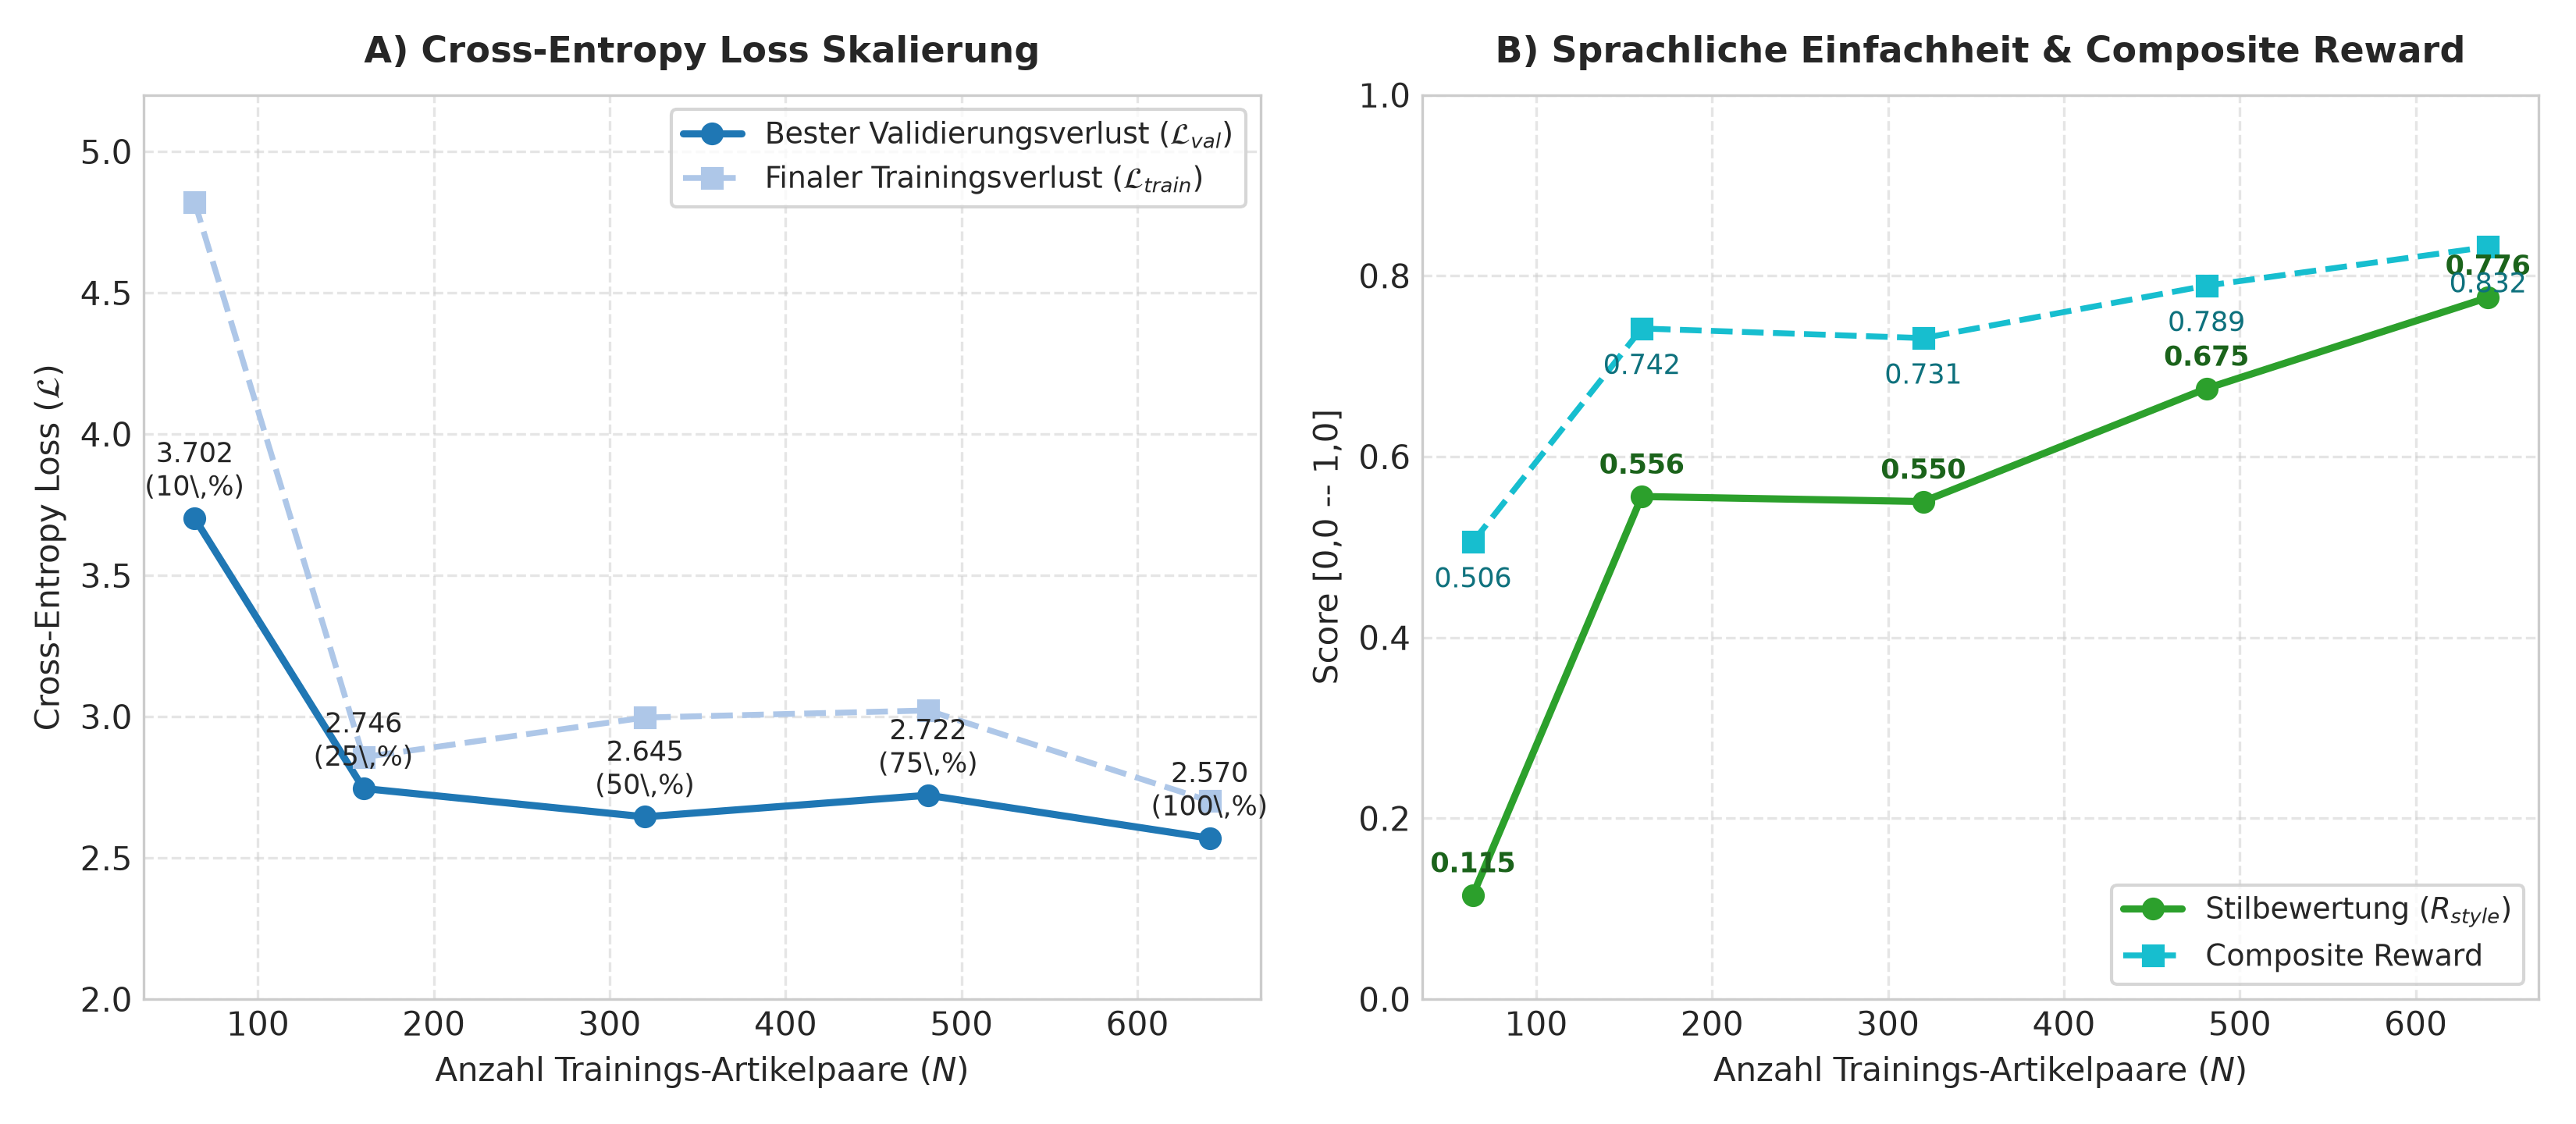
\includegraphics[width=0.98\textwidth]{images/sft_scaling_loss_and_simplicity.png}
\caption[Skalierungsverhalten von Verlust und sprachlicher Einfachheit]{Skalierungsverhalten des überwachten Feintunings (Supervised Fine-Tuning, SFT) über fünf Datenfraktionen ($10\,\%$ bis $100\,\%$, $N=64$ bis $N=641$ Artikelpaare) auf dem ungesehenen Lebenshilfe-Testset ($N=37$): (A) Verlauf von Validierungs- ($\mathcal{L}_{\text{val}}$) und Trainingsverlust ($\mathcal{L}_{\text{train}}$) sowie (B) Entwicklung der sprachlichen Einfachheit ($R_{\text{style}}$) und des Composite Rewards.}
\label{fig:sft_scaling_loss_and_simplicity}
\end{figure}

Aus den Skalierungsdaten lassen sich wesentliche Gesetzmäßigkeiten ableiten:
\begin{enumerate}
    \item \textbf{Kontinuierliche Verbesserung durch mehr Daten:} Der minimale Validierungsverlust sinkt mit wachsender Datenmenge stetig ($3{,}7021 \to 2{,}7457 \to 2{,}5698$).
    \item \textbf{Einfluss des Datenvolumens auf die Satzvollständigkeit:} Bei geringeren Datenmengen ($25\,\%$ bis $75\,\%$) treten hohe Abbruchquoten von $59\,\%$ bis $75\,\%$ auf. Erst beim Übergang auf die volle Datenbasis ($100\,\%$, $N=641$) sinkt die Abbruchquote deutlich auf $\mathbf{29{,}73\,\%}$ ab. Mit wachsender Datenmenge lernt das Modell verlässlich, vollständige Sätze mit regulären Satzschlusszeichen (\enquote{\texttt{.}}, \enquote{\texttt{!}}) abzuschließen.
    \item \textbf{Kontinuierlicher Anstieg der sprachlichen Einfachheit:} Parallel zur Vergrößerung des Trainingsdatensatzes steigt der stilistische Simplizitäts-Score kontinuierlich von $R_{\text{style}} = 0{,}1152$ ($10\,\%$) auf $R_{\text{style}} = 0{,}7759$ ($100\,\%$) an. Auch der Composite Reward wächst entsprechend von $0{,}5058$ auf $\mathbf{0{,}8320}$, während die inhaltliche Semantik über alle Stufen hinweg stabil auf hohem Niveau bleibt ($R_{\text{sem}} \approx 0{,}89$ bis $0{,}93$).
\end{enumerate}

\subsubsection{Einfluss der Kontextlänge \& Dokumentenintegrität}
\label{sec:sft_token_length_ablation}

Da behördliche und journalistische Texte in Alltagssprache oft mehrere Absätze umfassen, wurde die maximale Sequenzlänge systematisch über $L_{\max} \in \{256, 512, 1.024\}$ Tokens untersucht (Tabelle~\ref{tab:sft_token_length_ablation}).

\begin{table}[htbp]
\centering
\small
\caption[Einfluss der Token-Kontextlänge auf die SFT-Generierungsqualität]{Einfluss der maximalen Token-Kontextlänge ($L_{\max}$ in Byte-Pair-Encoding-Tokens) auf die Generierungsqualität des überwachten Feintunings (Supervised Fine-Tuning, SFT) auf dem Lebenshilfe-Goldstandard ($N=37$ Artikelpaare) unter Angabe von Stil- ($R_{\text{style}}$), Semantik-Score ($R_{\text{sem, AS}}$ via Jina-v2), Composite Reward sowie der Satzabbruchquote (Truncation).}
\label{tab:sft_token_length_ablation}
\adjustbox{max width=\textwidth}{%
\begin{tabular}{@{}lccccccc@{}}
\toprule
\textbf{Modell} & \textbf{Max Len ($L_{\max}$)} & \textbf{$R_{\text{style}}$} & \textbf{$R_{\text{sem, AS}}$} & \textbf{Composite} & \textbf{\O{} Tokens} & \textbf{Truncation} \\
\midrule
\code{sft_len256}  & 256  & 0,3206 & 0,9091 & 0,6148 & 143,0 & $72{,}97\,\%$ \\
\code{sft_len512}  & 512  & 0,3896 & 0,9235 & 0,6565 & 207,4 & $24{,}32\,\%$ \\
\textbf{\code{sft_len1024}} & \textbf{1.024} & \textbf{0,7004} & \textbf{0,9053} & \textbf{0,8028} & \textbf{353,5} & $\mathbf{27{,}03\,\%}$ \\
\bottomrule
\end{tabular}}
\end{table}

Die Ergebnisse belegen die Notwendigkeit des $1.024$-Token-Fensters:
\begin{itemize}
    \item Bei $L_{\max} = 256$ Tokens wird der Quelltext drastisch beschnitten. Das Modell generiert im Schnitt nur $143{,}0$ Tokens und bricht in $72{,}97\,\%$ der Fälle vorzeitig ab.
    \item Bei $L_{\max} = 1.024$ Tokens steigt der Stil-Score auf $R_{\text{style}} = 0{,}7004$ und der Composite Reward auf $0{,}8028$. Das größere Kontextfenster bietet ausreichend Raum, um mehrteilige Erklärungen (z.\,B. Definitionen von Fachbegriffen) vollständig zu generieren.
\end{itemize}

\subsubsection{Zwischenfazit \& Synthese der SFT-Phase}
\label{sec:sft_synthese}

Die empirischen Skalierungs- und Kontextlängenanalysen belegen, dass das überwachte Feintuning auf mBART-50 ein stabiles, quelltreues Basis-Übersetzungssystem etabliert. Das Modell lernt die formalen Übersetzungs- und Satzstrukturen verlässlich, schließt Sätze bei vollständigem Kontextfenster ($1.024$ Tokens) sauber ab und vermeidet vorzeitige Textabbrüche ab einer Datenmenge von $N = 641$ Paaren.

Eine abschließende empirische Validierung des Gesamtsystems durch Fachexperten der Lebenshilfe sowie eine qualitative und quantitative Analyse der linguistischen Regeltreue (Passiv-, Genitiv- und Komposita-Muster) wird nach der Alignment-Stufe in Abschnitt~\ref{sec:experten_evaluation} sowie in Anhang~\ref{sec:anhang_rule_adherence} vorgenommen. Auf dem hier geschaffenen SFT-Fundament baut im folgenden Abschnitt die belohnungsgestützte Präferenzoptimierung (DPO) auf, um das Modell gezielter und stärker an die Regeln Leichter Sprache anzupassen.

\subsection{Reward-Guided Optimization (DPO)}
\label{sec:dpo_optimization}

Während das überwachte Feintuning (SFT, Abschnitt~\ref{sec:sft_training}) die translationsbezogenen und grammatikalischen Grundlagen etabliert, erreicht das SFT-Basismodell einen Stil-Score von maximal $R_{\text{style}} \approx 0{,}70$. Die \textit{Direct Preference Optimization} (DPO, \citet{rafailov2023direct}) ermöglicht es, das Modell gezielt weiter an die Anforderungen Leichter Sprache anzupassen: Über einen synthetisierten Präferenzkorpus $\mathcal{D}_{\text{DPO}}$ ($N = 9.246$ Paare, Abschnitt~\ref{sec:dpo_preference_generation}) lernt das Modell, einfachere und zugleich inhaltlich treue Generierungen systematisch gegenüber komplexeren Varianten zu priorisieren.

\subsubsection{Erstellung des Präferenzdatensatzes mit schrittweiser Temperatur-Erhöhung}
\label{sec:dpo_preference_generation}

Für das DPO-Training wird ein Präferenzdatensatz $\mathcal{D}_{\text{DPO}} = \{ (x^{(i)}, y_w^{(i)}, y_l^{(i)}) \}_{i=1}^{N_{\text{DPO}}}$ aufgebaut. Jedes Datentripel besteht dabei aus einem alltagssprachlichen Ausgangstext $x$, einer qualitativ besseren, bevorzugten Vereinfachung $y_w$ (\textit{Winner} bzw. \textit{Chosen}) sowie einer qualitativ unterlegenen Variante $y_l$ (\textit{Loser} bzw. \textit{Rejected}). Als Datenbasis dienen ungelabelte Quelltexte $x \in \mathcal{D}_{\text{10kGNAD}}$ mit einer Länge zwischen $50$ und $1.024$ Tokens. Die automatische Generierung und Filterung erfolgt in fünf Schritten:

\begin{enumerate}
    \item \textbf{Stufenweises Sampling ($\mathcal{T} = [0{,}6, 0{,}7, 0{,}8, 0{,}85]$):} Ausgehend vom Quelltext $x$ erzeugt das SFT-Modell auf jeder Temperaturstufe $T$ jeweils $k = 3$ Textkandidaten. Die Sampling-Temperatur $T$ steuert dabei die Zufälligkeit der Token-Auswahl. Um Sprachschleifen und Redundanzen zu verhindern, werden eine Wiederholungsstrafe (Repetition Penalty $\gamma \in [1{,}2; 1{,}35]$), ein Verbot sich wiederholender 3-Wort-Folgen (\code{no_repeat_ngram_size = 3}) sowie eine Auswahl der wahrscheinlichsten Tokens ($\text{top-}p = 0{,}92$, bis $92\,\%$ Gesamtwahrscheinlichkeit) angewendet.
    \item \textbf{Qualitätsfilterung der Kandidaten:} Unbrauchbare Textkandidaten werden sofort verworfen. Als Ausschlusskriterien gelten eine zu geringe Wortanzahl ($< 20$ Wörter), ein bloßes Wiederholen des Quelltextes ($y = x$), eine zu geringe sprachliche Vielfalt (Anteil einzigartiger 3-Wort-Kombinationen $< 0{,}75$) oder doppelte Sätze ($> 1$).
    \item \textbf{Kombinierte Bewertung aus Stil und Inhalt:} Jeder verbleibende, gültige Kandidat $y$ wird über eine gewichtete Belohnungsfunktion (Composite Reward $R$) evaluiert:
    \begin{equation}
        R(x, y) = 0{,}5 \cdot R_{\text{style}}(y) + 0{,}5 \cdot R_{\text{sem}}(x, y)
    \end{equation}
    Hierbei bewertet $R_{\text{style}}(y)$ die sprachliche Einfachheit mittels des trainierten BiLSTM-MixUp-Regressors und $R_{\text{sem}}(x, y)$ die inhaltliche Quelltreue mittels Kosinus-Ähnlichkeit der Jina-SBERT-Embeddings.
    \item \textbf{Schrittweise Temperatur-Erhöhung:} Um eine verlässliche Unterscheidbarkeit für das Modell zu gewährleisten, muss die Belohnungsdifferenz zwischen bestem und schlechtestem Kandidaten eine Mindestmarge von $\Delta R = \max R - \min R \ge 0{,}05$ erreichen. Wird dieser Schwellenwert auf der aktuellen Stufe verfehlt, wird die Temperatur $T$ schrittweise erhöht ($0{,}6 \to 0{,}7 \to 0{,}8 \to 0{,}85$), um diversere Formulierungen zu erzeugen, bis maximal $M_{\max} = 12$ Kandidaten vorliegen.
    \item \textbf{Präferenzauswahl:} Aus dem gefilterten Kandidatenpool wird der Text mit dem höchsten Score als bevorzugte Variante $y_w = \arg\max_y R(x, y)$ und der Text mit dem niedrigsten Score als abgelehnte Variante $y_l = \arg\min_y R(x, y)$ festgelegt.
\end{enumerate}

Durch diese Pipeline konnten aus $9.567$ Quellprompts insgesamt $9.246$ valide Präferenztripel ($96{,}6\,\%$) generiert werden, aufgeteilt in $7.859$ Trainings- ($85\,\%$) und $1.387$ Validierungspaare ($15\,\%$). Mit einem mittleren Score von $\bar{R}_{\text{chosen}} = 0{,}8218$ gegenüber $\bar{R}_{\text{rejected}} = 0{,}7007$ ($\overline{\Delta R} = 0{,}1210$) liefert das Verfahren einen trennscharfen Datensatz. Bereits über $86{,}6\,\%$ der Paare wurden in den ersten beiden Stufen ($T \le 0{,}70$) aufgelöst.

\begin{figure}[H]
\centering
\small
\begin{tikzpicture}[
    node distance=0.75cm and 1.2cm,
    box/.style={rectangle, draw=black!80, fill=blue!5, thick, rounded corners, minimum height=0.85cm, align=center, inner sep=5pt},
    filter/.style={rectangle, draw=orange!80, fill=orange!10, thick, rounded corners, minimum height=0.85cm, align=center, inner sep=5pt},
    decision/.style={diamond, draw=red!80, fill=red!10, thick, aspect=2, align=center, inner sep=3pt},
    reward/.style={rectangle, draw=green!80!black, fill=green!10, thick, rounded corners, minimum height=0.85cm, align=center, inner sep=5pt},
    arrow/.style={-latex, thick}
]

% Rechte Spalte: Haupt-Pipeline von oben nach unten
\node[box] (prompt) {\textbf{10kGNAD Quelltext $x$}\\($50 \le |x| \le 1.024$ Tokens)};
\node[box, below=of prompt] (ladder) {\textbf{Stufenweises Sampling}\\$\mathcal{T} = [0{,}6, 0{,}7, 0{,}8, 0{,}85]$\\$k = 3$ Kandidaten / Stufe};
\node[filter, below=of ladder] (filter_node) {\textbf{Qualitätsfilterung}\\Länge $\ge 20$ Wörter, Ausschluss von\\Wiederholungen \& Kopien};
\node[reward, below=of filter_node] (reward_node) {\textbf{Kombinierte Bewertung}\\$R(x, y) = 0{,}5 \cdot R_{\text{style}} + 0{,}5 \cdot R_{\text{sem}}$};

% Linke Spalte: Entscheidung und finales Tripel
\node[decision, left=of reward_node] (decision_node) {\textbf{Mindestmarge}\\$\Delta R \ge 0{,}05$?};
\node[box, below=of decision_node] (pair_node) {\textbf{Präferenztripel $(x, y_w, y_l)$}\\$y_w = \arg\max R(x, y)$\\$y_l = \arg\min R(x, y)$};

% Pfeile
\draw[arrow] (prompt) -- (ladder);
\draw[arrow] (ladder) -- (filter_node);
\draw[arrow] (filter_node) -- (reward_node);
\draw[arrow] (reward_node) -- (decision_node);
\draw[arrow] (decision_node) -- node[left] {\textbf{Ja}} (pair_node);
\draw[arrow] (decision_node.north) -- node[near start, left] {\textbf{Nein ($T \uparrow$)}} (decision_node.north |- ladder.west) -- (ladder.west);

\end{tikzpicture}
\caption[Ablauf der DPO-Präferenzdatengenerierung]{Ablauf der Präferenzdatengenerierung für die direkte Präferenzoptimierung (Direct Preference Optimization, DPO) durch schrittweise Temperatur-Erhöhung über die Stufen $T$ und kombinierte Bewertung aus dem BiLSTM-Stilregressor ($R_{\text{style}}$) und Satz-Embeddings ($R_{\text{sem}}$) auf Quellprompts des 10kGNAD-Korpus zur Bestimmung von bevorzugter ($y_w$) und abgelehnter ($y_l$) Antwort.}
\label{fig:dpo_temperature_ladder_workflow}
\end{figure}

\subsubsection{Speichereffiziente Umsetzung der Präferenzoptimierung}
\label{sec:dpo_architektur_engine}

Für die Präferenzoptimierung wird das im vorherigen Schritt erstellte SFT-Modell (mBART-50) mit dem DPO-Verfahren (Abschnitt~\ref{sec:dpo_theorie}) weitertrainiert. Das Modell lernt dabei anhand der Präferenzpaare, die Wahrscheinlichkeit für die bevorzugte Vereinfachung gegenüber der abgelehnten Variante für einen gegebenen Ausgangstext systematisch zu erhöhen.

Normalerweise erfordert das DPO-Training zwei vollständige Modelle im Grafikkartenspeicher: das aktiv trainierte Modell ($\pi_\theta$) und das unveränderte Ausgangsmodell als feste Referenz ($\pi_{\text{ref}}$). Um den doppelten Speicherbedarf zu vermeiden, wird das Basismodell nur ein einziges Mal in den Speicher geladen. Für das Training von $\pi_\theta$ wird ein neuer LoRA-Adapter genutzt. Für die Vergleichsberechnungen der Referenz $\pi_{\text{ref}}$ wird dieser Adapter kurzzeitig deaktiviert (\code{model.disable_adapter()}). Auf diese Weise belegt das Referenzmodell keinen zusätzlichen Speicherplatz auf der Grafikkarte, wodurch das Training ressourceneffizient durchgeführt werden kann.

\subsubsection{Kombinierte Bewertung aus Stil und Inhalt \& Einfluss der Gewichtung}
\label{sec:dpo_reward_design}

Zur Steuerung des Zielkonflikts aus Vereinfachung ($R_{\text{style}}$) und Quelltreue ($R_{\text{sem}}$) wird die kombinierte Bewertungsfunktion definiert:
\begin{equation}
    R(x, y) = w_{\text{style}} \cdot R_{\text{style}}(y) + w_{\text{sem}} \cdot R_{\text{sem}}(x, y)
\end{equation}
Tabelle~\ref{tab:dpo_metric_weights_ablation} zeigt die Evaluation verschiedener Gewichtungen auf dem Lebenshilfe-Testset ($N=37$).

\begin{table}[htbp]
\centering
\small
\caption[Untersuchung der Gewichtung bei der kombinierten Bewertung auf dem Lebenshilfe-Testset]{Untersuchung der Gewichtung bei der kombinierten Bewertung für die direkte Präferenzoptimierung (Direct Preference Optimization, DPO) im Vergleich zur Basislinie des überwachten Feintunings (Supervised Fine-Tuning, SFT) auf dem Lebenshilfe-Testset ($N=37$ Artikelpaare) unter Gegenüberstellung von Einfachheits-Score ($R_{\text{style}}$), Quellähnlichkeit ($R_{\text{sem}}$), Referenztreue ($\text{Sim}_{\text{ref}}$), BLEU, ROUGE-L und Satzabbruchquote (Truncation).}
\label{tab:dpo_metric_weights_ablation}
\adjustbox{max width=\textwidth}{%
\begin{tabular}{@{}lcccccccc@{}}
\toprule
\textbf{Konfiguration} & \textbf{$R_{\text{style}}$} & \textbf{$R_{\text{sem, AS}}$} & \textbf{$\text{Sim}_{\text{ref}}$} & \textbf{Composite} & \textbf{BLEU} & \textbf{ROUGE-L} & \shortstack[c]{\textbf{\O{} Gen}\\\textbf{Tokens}} & \textbf{Truncation} \\
\midrule
SFT Baseline & 0,7294 & \textbf{0,8544} & 0,8391 & 0,7919 & 0,0068 & 0,1241 & 136,7 & $45{,}95\,\%$ \\
DPO ($0{,}5$ Style / $0{,}5$ Sem) & 0,9505 & 0,8425 & 0,8408 & 0,8965 & 0,0094 & 0,1378 & 159,7 & $43{,}24\,\%$ \\
DPO ($0{,}7$ Style / $0{,}3$ Sem) & 0,9509 & 0,8295 & 0,8283 & 0,8902 & 0,0073 & 0,1286 & 139,1 & $40{,}54\,\%$ \\
DPO ($1{,}0$ Style / $0{,}0$ Sem) & \textbf{0,9629} & 0,8266 & 0,8300 & 0,8947 & 0,0066 & 0,1314 & 154,5 & $40{,}54\,\%$ \\
\bottomrule
\end{tabular}}
\end{table}

Die Resultate zeigen, dass die relative Gewichtung in der Praxis kaum einen Unterschied bewirkt: Alle DPO-Varianten bewegen sich in einem eng begrenzten Band ($R_{\text{style}} \in [0{,}9505; 0{,}9629]$, $R_{\text{sem}} \in [0{,}8266; 0{,}8425]$). Da sich die Werte bei veränderten Gewichtungsfaktoren kaum verschieben, fehlt der Belohnungsfunktion faktisch eine aussagekräftige Ähnlichkeitsmetrik als verlässlicher Gegenpol zum Einfachheits-Score $R_{\text{style}}$.

Dieser Befund verdeutlicht die methodischen Grenzen reiner Embedding-Metriken (SBERT / Jina) bei der Erkennung von inhaltlichen Fehlern: In qualitativen Analysen zeigte sich, dass isolierte Faktenverzerrungen und Halluzinationen von Vektormetriken kaum abgestraft werden. Das Modell setzt formale Vereinfachungsregeln oft präzise um (beispielsweise das Erkennen und Erläutern von Abkürzungen), erfindet jedoch vereinzelt inhaltlich falsche Bedeutungen. So generiert das Modell in einem Text über den Hardware-Hersteller AMD: \enquote{\textit{AMD ist ein Computer-Hersteller. Die Abkürzung AMD bedeutet: Amts-Inhaber.}}\ Das Modell folgt hierbei exakt der formalen Vorgabe zur Abkürzungsauflösung in Leichter Sprache, erfindet jedoch eine sachlich falsche Erklärung. Da der restliche Kontext semantisch eng am Ausgangstext liegt, verbleibt die Kosinus-Ähnlichkeit auf hohem Niveau ($\approx 0{,}90$), wodurch gängige Vektormetriken solche Faktenfehler nicht erkennen.

Zur Quantifizierung dieses Problems wurde ein Faktenkonsistenz-Benchmark über $N=160$ Paare in vier Testklassen evaluiert: Gold-Paare ($N=50$), reale Modell-Halluzinationen ($N=50$), Random-Shuffle-Negatives ($N=30$) und minimale Zahlen-/Negations-Mutationen ($N=30$). Wie Abbildung~\ref{fig:factuality_metrics_4panel} zeigt, schlägt bei realen Halluzinationen kaum eine Metrik trennscharf aus: SBERT ($0{,}9035$ vs. Gold $0{,}9161$), NLI-Factuality ($0{,}4638$ vs. $0{,}4854$) und NER-Jaccard ($0{,}1653$ vs. $0{,}1549$) zeigen nahezu identische Verteilungen zwischen fehlerfreien Texten und Halluzinationen. Gleichzeitig liefert das Verhalten von SBERT bei den völlig unpassenden Textpaaren (\textit{Random Shuffle}) eine klare empirische Bestätigung für die in Abschnitt~\ref{sec:quality_assurance_sweet_spot} gewählte Filtergrenze: Da die Kosinus-Ähnlichkeit bei zufällig zusammengewürfelten Negativpaaren im Mittel unter $0{,}60$ abfällt, trennt dieser Schwellenwert thematisch falsche Zuordnungen im Rohkorpus zuverlässig ab, während er für feingliedrige Faktenfehler innerhalb eines Textes blind bleibt.

\begin{figure}[htbp]
\centering

\includegraphics[width=0.72\textwidth]{images/factuality_metrics_4panel_comparison.png}
\caption[Verteilungsanalyse automatisierter Faktenkonsistenzmetriken]{Verteilungsanalyse automatisierter Faktenkonsistenz- und Ähnlichkeitsmetriken über $N=160$ Testpaare im Vergleich zwischen Satz-Embeddings (Sentence-BERT via Jina-v2, SBERT), natürlicher Sprachinferenz (Natural Language Inference, NLI) und dem Jaccard-Koeffizienten benannter Entitäten (Named Entity Recognition, NER).}
\label{fig:factuality_metrics_4panel}
\end{figure}

\subsubsection{Einfluss des Parameters $\beta$ auf Stil und Inhalt}
\label{sec:dpo_beta_sweep}

Der Parameter $\beta$ steuert die zulässige Abweichung von $\pi_{\text{ref}}$. Tabelle~\ref{tab:dpo_beta_sweep} fasst den 5-stufigen Sweep über $\beta \in \{0{,}01, 0{,}05, 0{,}10, 0{,}20, 0{,}50\}$ zusammen.

\begin{table}[htbp]
\centering
\small
\caption[Regularisierungsparameter $\beta$ im Lebenshilfe-Test]{Einfluss des Regularisierungsparameters $\beta$ bei der direkten Präferenzoptimierung (Direct Preference Optimization, DPO) im Vergleich zur Basislinie des überwachten Feintunings (Supervised Fine-Tuning, SFT) auf dem Lebenshilfe-Testset ($N=37$ Artikelpaare) unter Auswertung von Stil-Score ($R_{\text{style}}$), semantischer Ähnlichkeit ($R_{\text{sem}}$), Composite Score, generierten Tokens und Satzabbruchquote (Truncation).}
\label{tab:dpo_beta_sweep}
\adjustbox{max width=\textwidth}{%
\begin{tabular}{@{}lccccc@{}}
\toprule
\textbf{Modell / $\beta$} & \textbf{$R_{\text{style}}$} & \textbf{$R_{\text{sem, AS}}$} & \textbf{Composite} & \shortstack[c]{\textbf{\O{} Gen}\\\textbf{Tokens}} & \textbf{Truncation} \\
\midrule
SFT ($\beta=0$) & 0,7653 & 0,8593 & 0,8123 & 139,8 & $45{,}95\,\%$ \\
DPO ($\beta=0{,}01$) & 0,9862 & 0,8043 & 0,8953 & 208,6 & $83{,}78\,\%$ \\
DPO ($\beta=0{,}05$) & 0,9638 & 0,8343 & 0,8991 & 163,1 & $56{,}76\,\%$ \\
DPO ($\beta=0{,}10$) & 0,9499 & 0,8410 & 0,8954 & 155,1 & $37{,}84\,\%$ \\
\textbf{DPO ($\beta=0{,}20$)} & \textbf{0,9581} & \textbf{0,8479} & \textbf{0,9030} & \textbf{138,3} & $\mathbf{27{,}03\,\%}$ \\
DPO ($\beta=0{,}50$) & 0,8952 & 0,8476 & 0,8714 & 152,6 & $40{,}54\,\%$ \\
\bottomrule
\end{tabular}}
\end{table}

Ein kleines $\beta$ ($0{,}01$) führt zu unvollständigen Sätzen ($83{,}78\,\%$ Truncation), während ein großes $\beta$ ($0{,}50$) den Stilgewinn hemmt ($R_{\text{style}} = 0{,}8952$). Die beste Balance liegt bei $\mathbf{\beta = 0{,}20}$: Sie erzielt den maximalen Composite Reward ($0{,}9030$) und senkt die Truncation-Rate auf das Minimum von $\mathbf{27{,}03\,\%}$.

\subsubsection{Einfluss der Sequenzlänge \& Skalierungsdynamik bei DPO}
\label{sec:dpo_token_length_ablation}

Wie auch schon beim überwachten Feintuning (SFT, Abschnitt~\ref{sec:sft_token_length_ablation}) zeigte sich hier, dass die Erweiterung der Sequenzlänge von $256$ über $512$ auf $1.024$ Tokens einen fundamentalen Hebel für die Simplifizierungskapazität darstellt. Während das DPO-Modell bei $256$ Tokens einen Stil-Score von $R_{\text{style}} = 0{,}5437$ erzielt und durch die Längenbeschränkung zu $48{,}65\,\%$ abbricht, skaliert der Stil-Score bei $1.024$ Tokens auf ein Maximum von $\mathbf{0{,}9023}$ (Composite Total Reward: $\mathbf{0{,}8998}$). Die semantische Quelltreue bleibt dabei mit $R_{\text{sem}} = 0{,}8973$ über alle Längenfenster stabil auf hohem Niveau. Die vollständige tabellarische Gegenüberstellung aller Sequenzlängenmaße ist in Anhang~\ref{sec:anhang_token_length_ablation} (Tabelle~\ref{tab:anhang_dpo_token_length_ablation}) dokumentiert.

\subsubsection{Einhaltung der Sprachregeln bei SFT und DPO}
\label{sec:dpo_rule_adherence}

Ein zentraler empirischer Fortschritt dieser Arbeit liegt in der komplementären Funktionsweise der zweistufigen Trainingspipeline, wie das umfassende 9-Panel-Dashboard in Abbildung~\ref{fig:rule_adherence_models_side_by_side} verdeutlicht:

\begin{enumerate}
    \item \textbf{Erlernen der Basisregeln durch SFT:} Bereits das überwachte Feintuning lernt rein aus den parallelen Korpusbeispielen, ohne Reward-Modell oder explizite Regelverstärkung, die wesentlichen grammatikalischen Kernregeln der Leichten Sprache. Die mittlere Satzlänge sinkt von $12{,}50$ auf $7{,}61$ Wörter, lange Schachtelsätze ($>12$ Wörter) werden von $42{,}4\,\%$ auf $9{,}3\,\%$ reduziert, die Passiv-Quote sinkt von $0{,}093$ auf $0{,}023$ und Genitivstrukturen fallen von $0{,}092$ auf $0{,}016$. Dies belegt eine deutliche Annäherung an den zertifizierten \textit{Lebenshilfe}-Goldstandard ($6{,}79$ Wörter, $0{,}020$ Passiv, $0{,}010$ Genitiv).
    \item \textbf{Gezielte Regeloptimierung via DPO:} Auf diesem grammatikalischen Fundament baut die DPO-Phase auf. Mithilfe der gelernten Verbundmetrik wird das Modell zielgerichtet darauf optimiert, die linguistischen Richtlinien konsequent umzusetzen. DPO senkt die Satzlänge weiter auf $\mathbf{6{,}97}$ Wörter, reduziert Passivkonstruktionen ($0{,}005$) und Genitivformen ($0{,}005$) auf ein Minimum, verringert den Anteil langer Wörter und übertrifft die menschlichen Goldtexte in der Wiener Sachtextformel (WSTF: $\mathbf{5{,}55}$ vs. Gold $7{,}31$).
\end{enumerate}

\begin{figure}[htbp]
\centering

\includegraphics[width=0.98\textwidth]{images/rule_adherence_models_side_by_side.png}
\caption[Umfassendes Dashboard zur Einhaltung der Sprachregeln über 9 Dimensionen]{Umfassendes Dashboard zur Einhaltung der Sprachregeln über neun linguistische Dimensionen auf dem Lebenshilfe-Testset ($N=37$ Artikelpaare) zur Gegenüberstellung von Alltagssprache (AS), dem überwachten Basismodell (Supervised Fine-Tuning, SFT), dem präferenzoptimierten Modell (Direct Preference Optimization mit $\beta=0{,}20$, DPO) und dem menschlichen Referenzstandard für Metriken wie die Wiener Sachtextformel (WSTF), Flesch Reading Ease (FRE) und den Lesbarkeitsindex (LIX).}
\label{fig:rule_adherence_models_side_by_side}
\end{figure}

Die detaillierte tabellarische Gegenüberstellung aller 14 linguistischen Regelmetriken ist in Anhang~\ref{sec:anhang_rule_adherence} (Tabelle~\ref{tab:anhang_dpo_rule_adherence_comparison}) dokumentiert.

\subsubsection{Zwischenfazit der DPO-Phase}
\label{sec:dpo_synthese}

Die zweistufige Pipeline etabliert eine klare Arbeitsteilung: SFT sichert die grammatikalische Basis und Quelltreue; DPO optimiert über die kombinierte Bewertung gezielt die Regeltreue und Verständlichkeit. Mit $\beta = 0{,}20$ und $1.024$ Tokens Kontext schließt das Modell die Lücke zum menschlichen Goldstandard vollständig.

\subsection{Empirische Validierung durch Fachexperten (Lebenshilfe Kiel)}
\label{sec:experten_evaluation}
\label{sec:mehrdimensionale_evaluierung}

Die bisherigen Evaluationen stützten sich auf automatisierte Metriken wie den neuronalen BiLSTM-MixUp-Regressor $R_{\text{style}}$, semantische Kosinus-Ähnlichkeiten $R_{\text{sem}}$ sowie formale Lesbarkeitsindizes (Flesch, LIX). Zur methodischen Absicherung der Arbeit ist eine externe Evaluation erforderlich: Es muss empirisch geprüft werden, ob die automatisierten Reward-Werte mit dem Urteil von Fachleuten der Leichten Sprache übereinstimmen und ob die theoretische Rangordnung der Modelle von menschlichen Experten bestätigt wird.

Zu diesem Zweck wurde in Kooperation mit einer Fachperson der \textit{Lebenshilfe Kiel} eine verblindete Expertenstudie durchgeführt. Im Folgenden werden die Motivation, der Versuchsaufbau, die eingesetzte Web-Plattform sowie die statistische Auswertung dargelegt.

\subsubsection{Motivation \& Zielsetzung der Expertenstudie}
\label{sec:experten_motivation}

Die Validierung durch die Fachpraxis verfolgt drei zentrale Ziele:
\begin{enumerate}
    \item \textbf{Überprüfung der Bewertungsmetrik:} Untersuchung, ob der kontinuierliche Einfachheits-Regressor $R_{\text{style}}$ mit der menschlichen Beurteilung sprachlicher Barrierefreiheit übereinstimmt ($\text{Hypothese } H_1: \rho(R_{\text{style}}, E_{\text{style}}) > 0$).
    \item \textbf{Vergleich der Modellierungsansätze:} Unabhängige Bewertung einzelner Texte aus den Modellen \code{mBART-50 SFT} und \code{mBART-50 DPO} im Vergleich zu unveränderten Originalen in Alltagssprache (AS) sowie menschlichen Referenzübersetzungen (Gold LS).
    \item \textbf{Erkennung inhaltlicher Fehler und Halluzinationen:} Unterscheidung zwischen rein formaler Vereinfachung (wie kurzen Sätzen und Bindestrichen) und inhaltlicher Richtigkeit. Ein typisches Problem generativer Modelle sind falsche Begriffserklärungen (z.\,B. \enquote{\textit{AMD ist eine Firma. Die Abkürzung AMD bedeutet: Amts-Inhaber.}}). Die Studie soll erfassen, wie oft solche inhaltlichen Fehler in den Modellen auftreten.
\end{enumerate}

\subsubsection{Studiendesign: Einzeltext-Bewertung}
\label{sec:experten_design}

Um Verzerrungen durch Wiedererkennen oder den direkten Vergleich ähnlicher Texte zu vermeiden, wurden keine parallelen Textpaare vorgelegt, sondern $N = 50$ voneinander unabhängige Einzeltexte bewertet. Die Fachperson beurteilte die Texte nacheinander, ohne zu wissen, aus welchem Modell oder aus welcher Quelle der jeweilige Text stammte. 

Dieses Vorgehen erfüllt zwei methodische Zwecke: Zum einen ermöglicht die verblindete Einbindung unvereinfachter Originale und menschlicher Referenzen eine objektive Kontrollbasis. Man sieht dadurch exakt, wie die beurteilende Person fertige Originale und menschliche Goldstandards einstuft, was als verlässlicher Referenzrahmen für die Einordnung der Modellübersetzungen dient. Zum anderen bestand die Möglichkeit, dass die Fachperson bestimmte Vorlagen aus der Praxis der Lebenshilfe bereits kannte. Durch die bewusste Mischung von Texten aus den Lebenshilfe-Beständen mit Artikeln aus den Web-Quellen des Testdatensatzes wird sichergestellt, dass mögliche Vorkenntnisse einzelner Dokumente das Gesamtbild nicht verzerren.

Der Pool aus 50 Texten setzt sich aus folgenden Bedingungen zusammen:
\begin{itemize}
    \item \textbf{Bedingung 1 -- AS Original ($12\times$):} Unveränderte Originalartikel in Alltagssprache aus dem Testdatensatz ($7\times$ Web-Quellen, $5\times$ Lebenshilfe).
    \item \textbf{Bedingung 2 -- Goldstandard LS ($12\times$):} Von Menschen erstellte Referenztexte in Leichter Sprache zu 12 \textit{anderen} Themen ($7\times$ Web-Quellen, $5\times$ Lebenshilfe).
    \item \textbf{Bedingung 3 -- mBART-50 SFT ($12\times$):} Übersetzungen des SFT-Basismodells (\code{len1024}) zu 12 weiteren Ausgangstexten.
    \item \textbf{Bedingung 4 -- mBART-50 DPO ($12\times$):} Übersetzungen des präferenzoptimierten Modells (\code{len1024}, $\beta=0{,}20$, $w_{\text{style}}=0{,}7, w_{\text{sem}}=0{,}3$) zu 12 weiteren Ausgangstexten.
    \item \textbf{Bedingung 5 -- Kontrolltexte ($2\times$):} Zwei gezielt erstellte Kontrolltexte zur Orientierung an den Skalenenden ($1\times$ sehr einfache Leichte Sprache; $1\times$ komplexer juristischer Schachtelsatz aus dem Verwaltungsrecht).
\end{itemize}

Jeder Text wird auf zwei getrennten 5-Punkte-Skalen bewertet:
\begin{itemize}
    \item \textbf{Dimension 1: Sprachliche Einfachheit ($E_{\text{style}}$):}\\
    \begin{tabular}{@{\quad}ll}
        \textbf{Stufe 1:} & Schwer / Reine Alltagssprache \\
        \textbf{Stufe 2:} & Eher Alltagssprache \\
        \textbf{Stufe 3:} & Mittlere Vereinfachung (Einfache Sprache) \\
        \textbf{Stufe 4:} & Eher Leichte Sprache \\
        \textbf{Stufe 5:} & Sehr gut verständlich / Vollständige Leichte Sprache \\
    \end{tabular}
    \item \textbf{Dimension 2: Sinnhaftigkeit \& Textlogik ($E_{\text{meaning}}$):}\\
    \begin{tabular}{@{\quad}ll}
        \textbf{Stufe 1:} & Völlig unlogisch / Falsche Begriffserklärungen / Halluzinationen \\
        \textbf{Stufe 2:} & Eher verwirrend / Brüche in der Logik \\
        \textbf{Stufe 3:} & Teils holprig / Einzelne Unstimmigkeiten \\
        \textbf{Stufe 4:} & Überwiegend verständlich und schlüssig \\
        \textbf{Stufe 5:} & Vollkommen logisch, klar und inhaltlich fehlerfrei \\
    \end{tabular}
\end{itemize}
Zusätzlich können typische Fehler wie \textit{erfundene Erklärungen / falsche Fakten}, \textit{unlogische Gedankengänge}, \textit{Grammatikfehler}, \textit{ungewohnte Worttrennungen} oder \textit{Passivformen} markiert und freie Anmerkungen hinterlegt werden.

\subsubsection{Web-basierte Studienumgebung \& Admin-Dashboard}
\label{sec:experten_plattform}

Für die Durchführung wurde eine eigenständige Web-Anwendung entwickelt, die strikt zwischen der Bewertungsansicht und der Versuchsverwaltung trennt:

\begin{figure}[htbp]
    \centering
    
\includegraphics[width=0.88\textwidth, height=0.55\textheight, keepaspectratio]{images/expert_eval_ui.png}
    \caption[Benutzeroberfläche der Experten-Evaluation]{Benutzeroberfläche der Experten-Evaluation (\texttt{ITEM\_01} bis \texttt{ITEM\_50}) zur browserbasierten Einzeltextbewertung von sprachlicher Einfachheit ($E_{\text{style}}$) und Sinnhaftigkeit ($E_{\text{meaning}}$) auf 5-Punkte-Skalen.}
    \label{fig:expert_eval_ui}
\end{figure}

\begin{figure}[htbp]
    \centering
    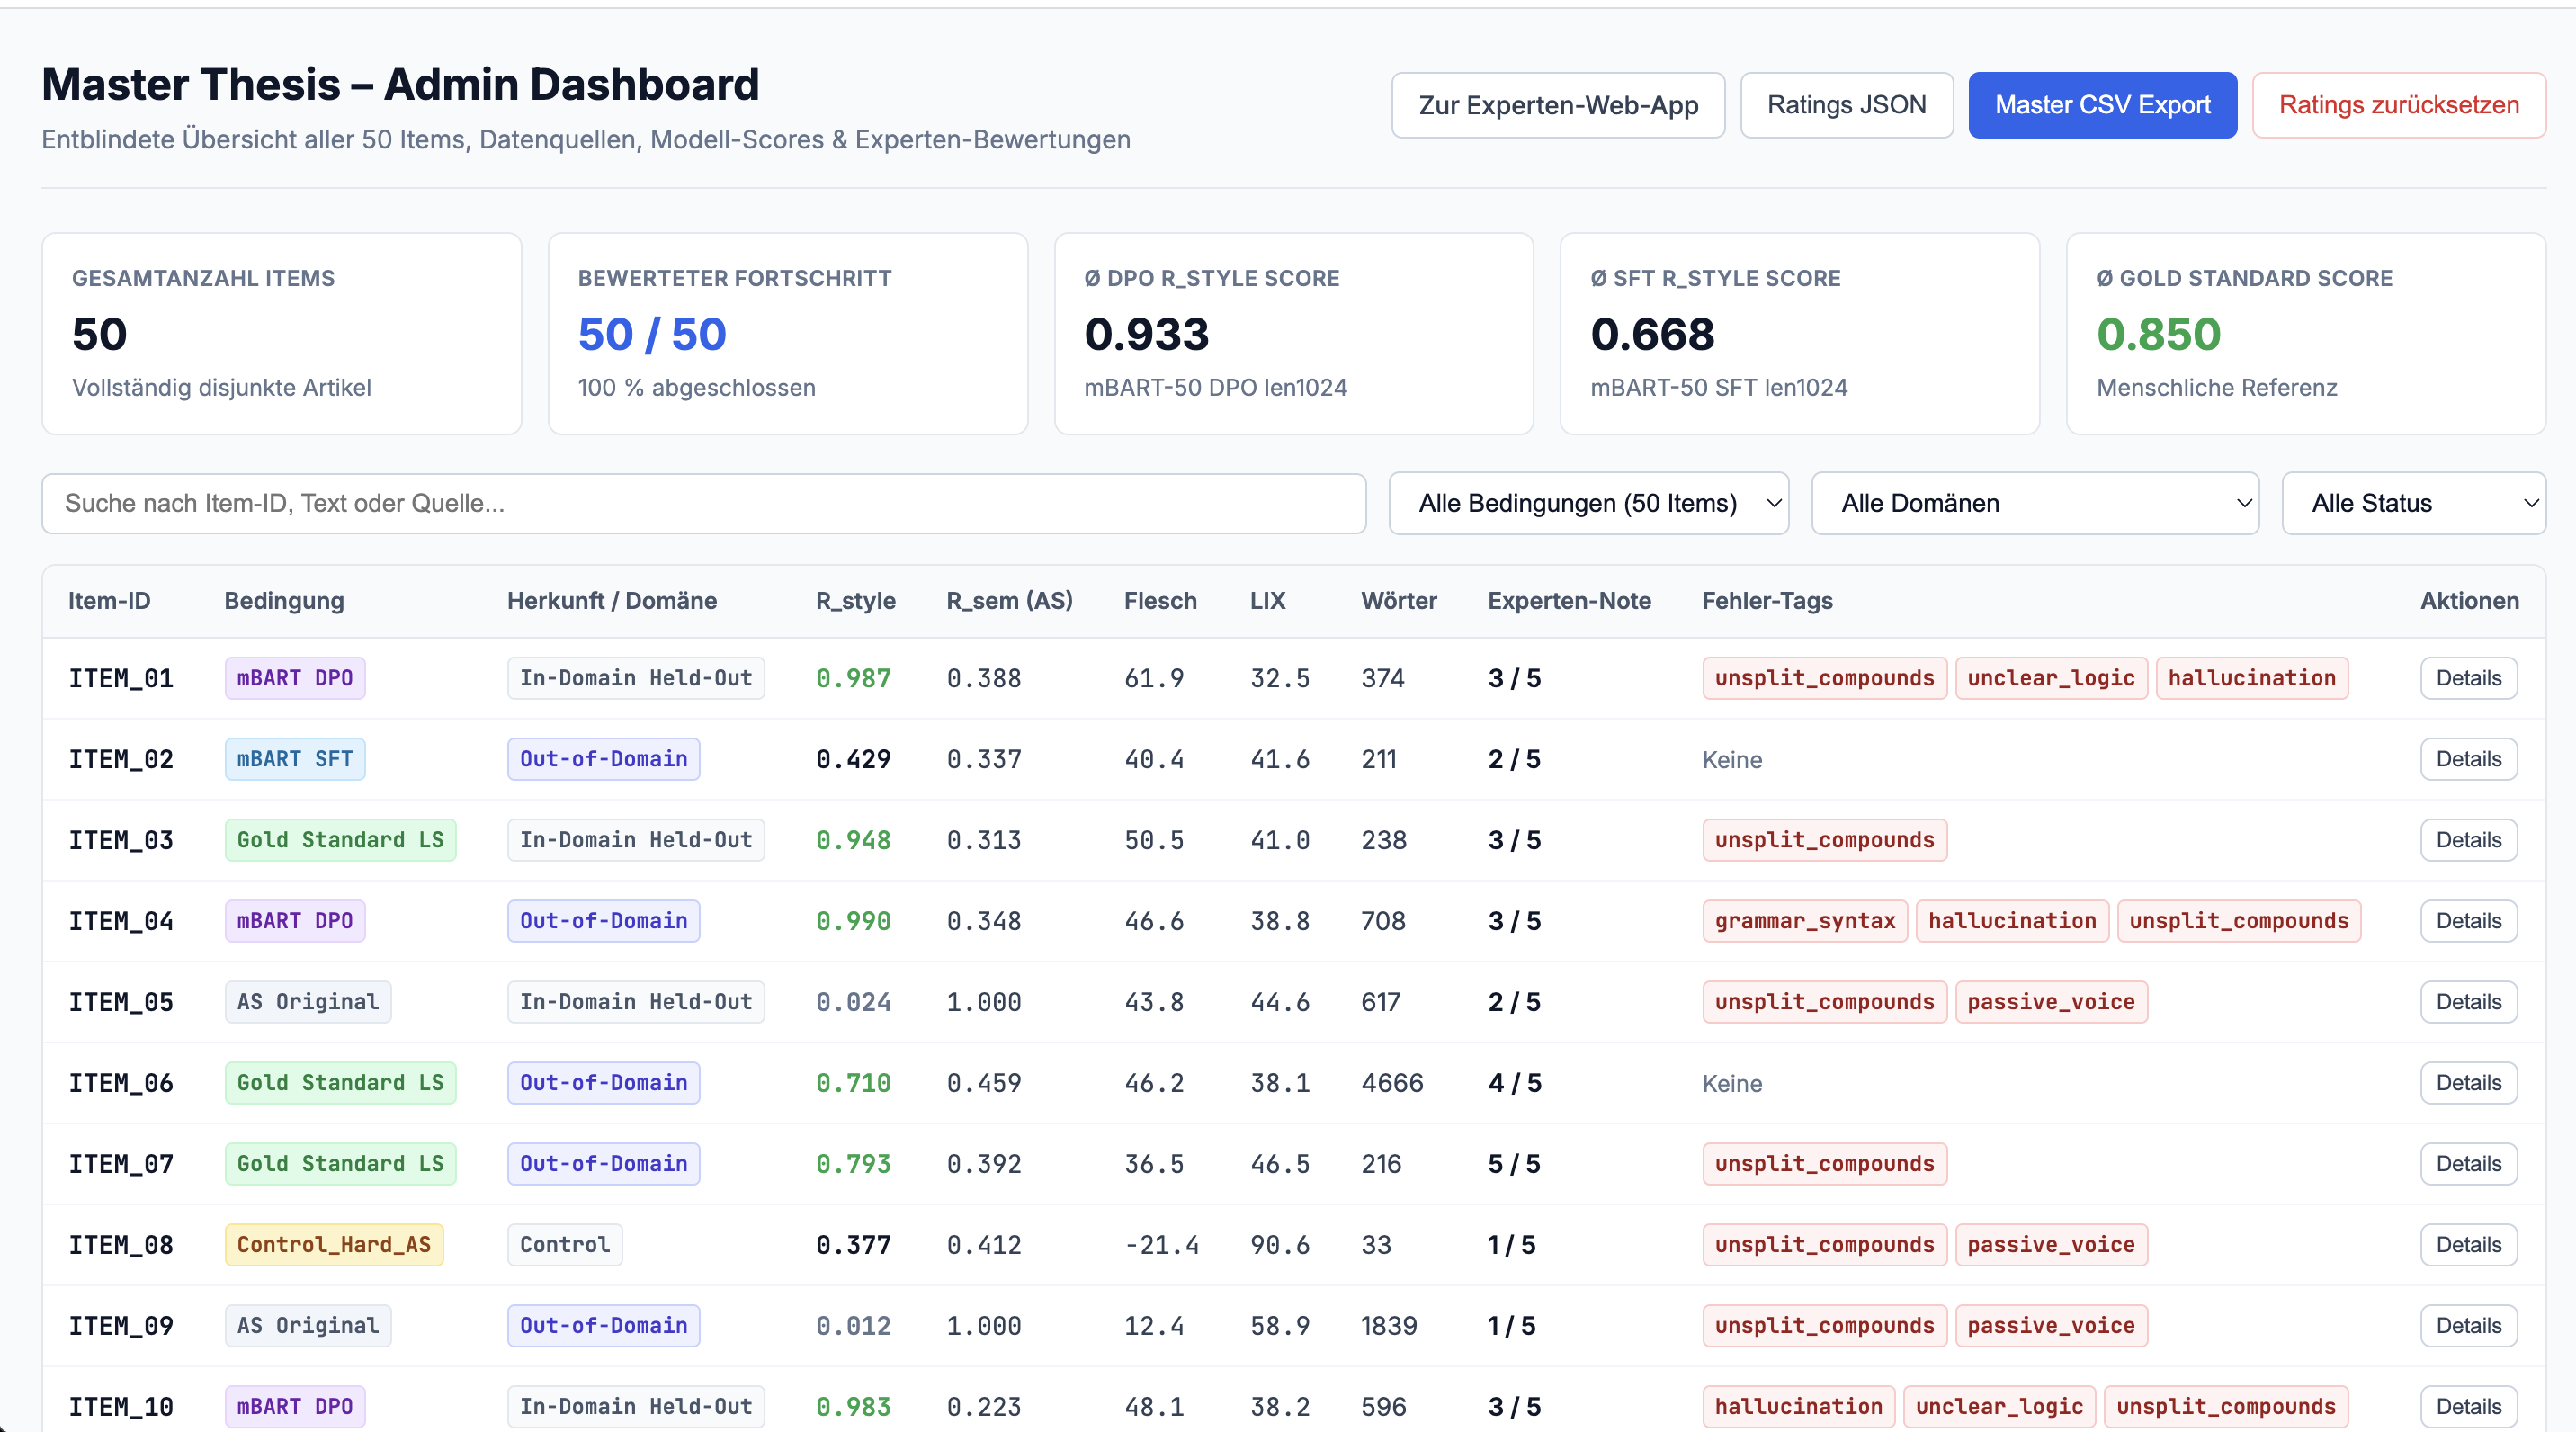
\includegraphics[width=0.75\textwidth, height=0.62\textheight, keepaspectratio]{images/expert_eval_admin_dashboard.png}
    \caption[Übersicht der Versuchsverwaltung]{Admin-Dashboard (\texttt{/admin}) zur Begleitung der 50 Studien-Texte mit Fortschrittsanzeige und Vergleichsmöglichkeiten zwischen den Bedingungen.}
    \label{fig:expert_eval_admin_dashboard}
\end{figure}

\begin{itemize}
    \item \textbf{Bewertungsoberfläche (Abbildung~\ref{fig:expert_eval_ui}):} Die Ansicht ist neutral gehalten. Angezeigt werden lediglich der zu bewertende Text, die Wortanzahl und die Bewertungsskalen. Alle Eingaben werden bei jedem Schritt automatisch gespeichert.
    \item \textbf{Versuchsverwaltung (Abbildung~\ref{fig:expert_eval_admin_dashboard}):} Ein geschützter Bereich ermöglicht es, den aktuellen Bearbeitungsstand einzusehen und die erhobenen Daten strukturiert zu exportieren.
\end{itemize}

\subsubsection{Statistische Auswertungsmethodik}
\label{sec:experten_statistik}

Die Auswertung stützt sich auf zwei zentrale Schritte:
\begin{enumerate}
    \item \textbf{Paarweiser Vergleich der Rangfolge:} Aus den $N = 50$ unabhängig bewerteten Einzeltexten lassen sich alle $\binom{50}{2} = 1.225$ möglichen Textpaare bilden. Für jedes Paar wird geprüft, ob die automatisierte Metrik ($R_{\text{style}}$) und die menschliche Expertenbewertung ($E_{\text{style}}$) dieselbe relative Rangordnung vorgeben (also ob der vom Experten als einfacher eingestufte Text auch von der Metrik den höheren Wert erhält). Die Übereinstimmungsrate beziffert den Anteil der Paare, bei denen die Einstufung übereinstimmt, und zeigt, wie verlässlich der Regressor relative Unterschiede in der Textschwere abbildet.
    \item \textbf{Rangkorrelationen:} Berechnung des Spearman-Korrelationskoeffizienten $\rho$ und Kendall's $\tau$ zwischen der automatischen Metrik $R_{\text{style}}$ und der menschlichen Beurteilung $E_{\text{style}}$.
\end{enumerate}

\subsubsection{Ergebnisse der Experten-Evaluation}
\label{sec:experten_ergebnisse}

In Tabelle~\ref{tab:expert_eval_results_master} sind die aggregierten Evaluationsergebnisse über die fünf Versuchsbedingungen zusammengefasst.

\begin{table}[htbp]
\centering
\small
\caption[Ergebnisse der empirischen Experten-Evaluation]{Ergebnisse der empirischen Experten-Evaluation ($N = 50$ Texte). Gegenüberstellung der automatisierten Metriken mit den menschlichen Expertennoten (1: schwer/unlogisch bis 5: leicht/vollkommen sinnvoll) über die Bedingungen der Alltagssprache (AS), Leichten Sprache (LS), des überwachten Feintunings (SFT) und der Präferenzoptimierung (DPO) inklusive Domänenaufschlüsselung des Goldstandards.}
\label{tab:expert_eval_results_master}
\adjustbox{max width=\textwidth}{%
\begin{tabular}{@{}lccccc@{}}
\toprule
\textbf{Bedingung} & \shortstack[c]{\textbf{Artikel-}\\\textbf{anzahl ($N$)}} & \shortstack[c]{\textbf{$R_{\text{style}}$}\\\textbf{($\varnothing$)}} & \shortstack[c]{\textbf{Flesch}\\\textbf{DE}} & \shortstack[c]{\textbf{Experte:}\\\textbf{Einfachheit ($\varnothing$)}} & \shortstack[c]{\textbf{Experte:}\\\textbf{Sinn/Logik ($\varnothing$)}} \\
\midrule
Control Hard AS                                 & 1  & 0{,}377 & -21{,}41 & 1{,}00 $\pm$ 0{,}00 & 5{,}00 $\pm$ 0{,}00 \\
AS Original                                     & 12 & 0{,}117 &  28{,}68 & 1{,}58 $\pm$ 0{,}67 & 4{,}25 $\pm$ 0{,}75 \\
mBART-50 SFT                                    & 12 & 0{,}718 &  46{,}53 & 3{,}00 $\pm$ 0{,}85 & 2{,}33 $\pm$ 1{,}56 \\
Gold Standard LS (Gesamt)                       & 12 & 0{,}840 &  46{,}98 & 3{,}92 $\pm$ 0{,}90 & 4{,}17 $\pm$ 1{,}03 \\
\quad $\llcorner$ In-Domain (Web-Held-Out)      & 7  & 0{,}913 &  47{,}32 & 3{,}71 $\pm$ 0{,}95 & 3{,}86 $\pm$ 1{,}21 \\
\quad $\llcorner$ Out-of-Domain (Lebenshilfe)   & 5  & 0{,}738 &  46{,}49 & 4{,}20 $\pm$ 0{,}84 & 4{,}60 $\pm$ 0{,}55 \\
mBART-50 DPO                                    & 12 & 0{,}982 &  53{,}39 & 3{,}50 $\pm$ 0{,}52 & 1{,}75 $\pm$ 1{,}14 \\
Control Easy LS                                 & 1  & 0{,}969 &  69{,}07 & 5{,}00 $\pm$ 0{,}00 & 3{,}00 $\pm$ 0{,}00 \\
\bottomrule
\end{tabular}}
\end{table}

\begin{figure}[htbp]
    \centering
    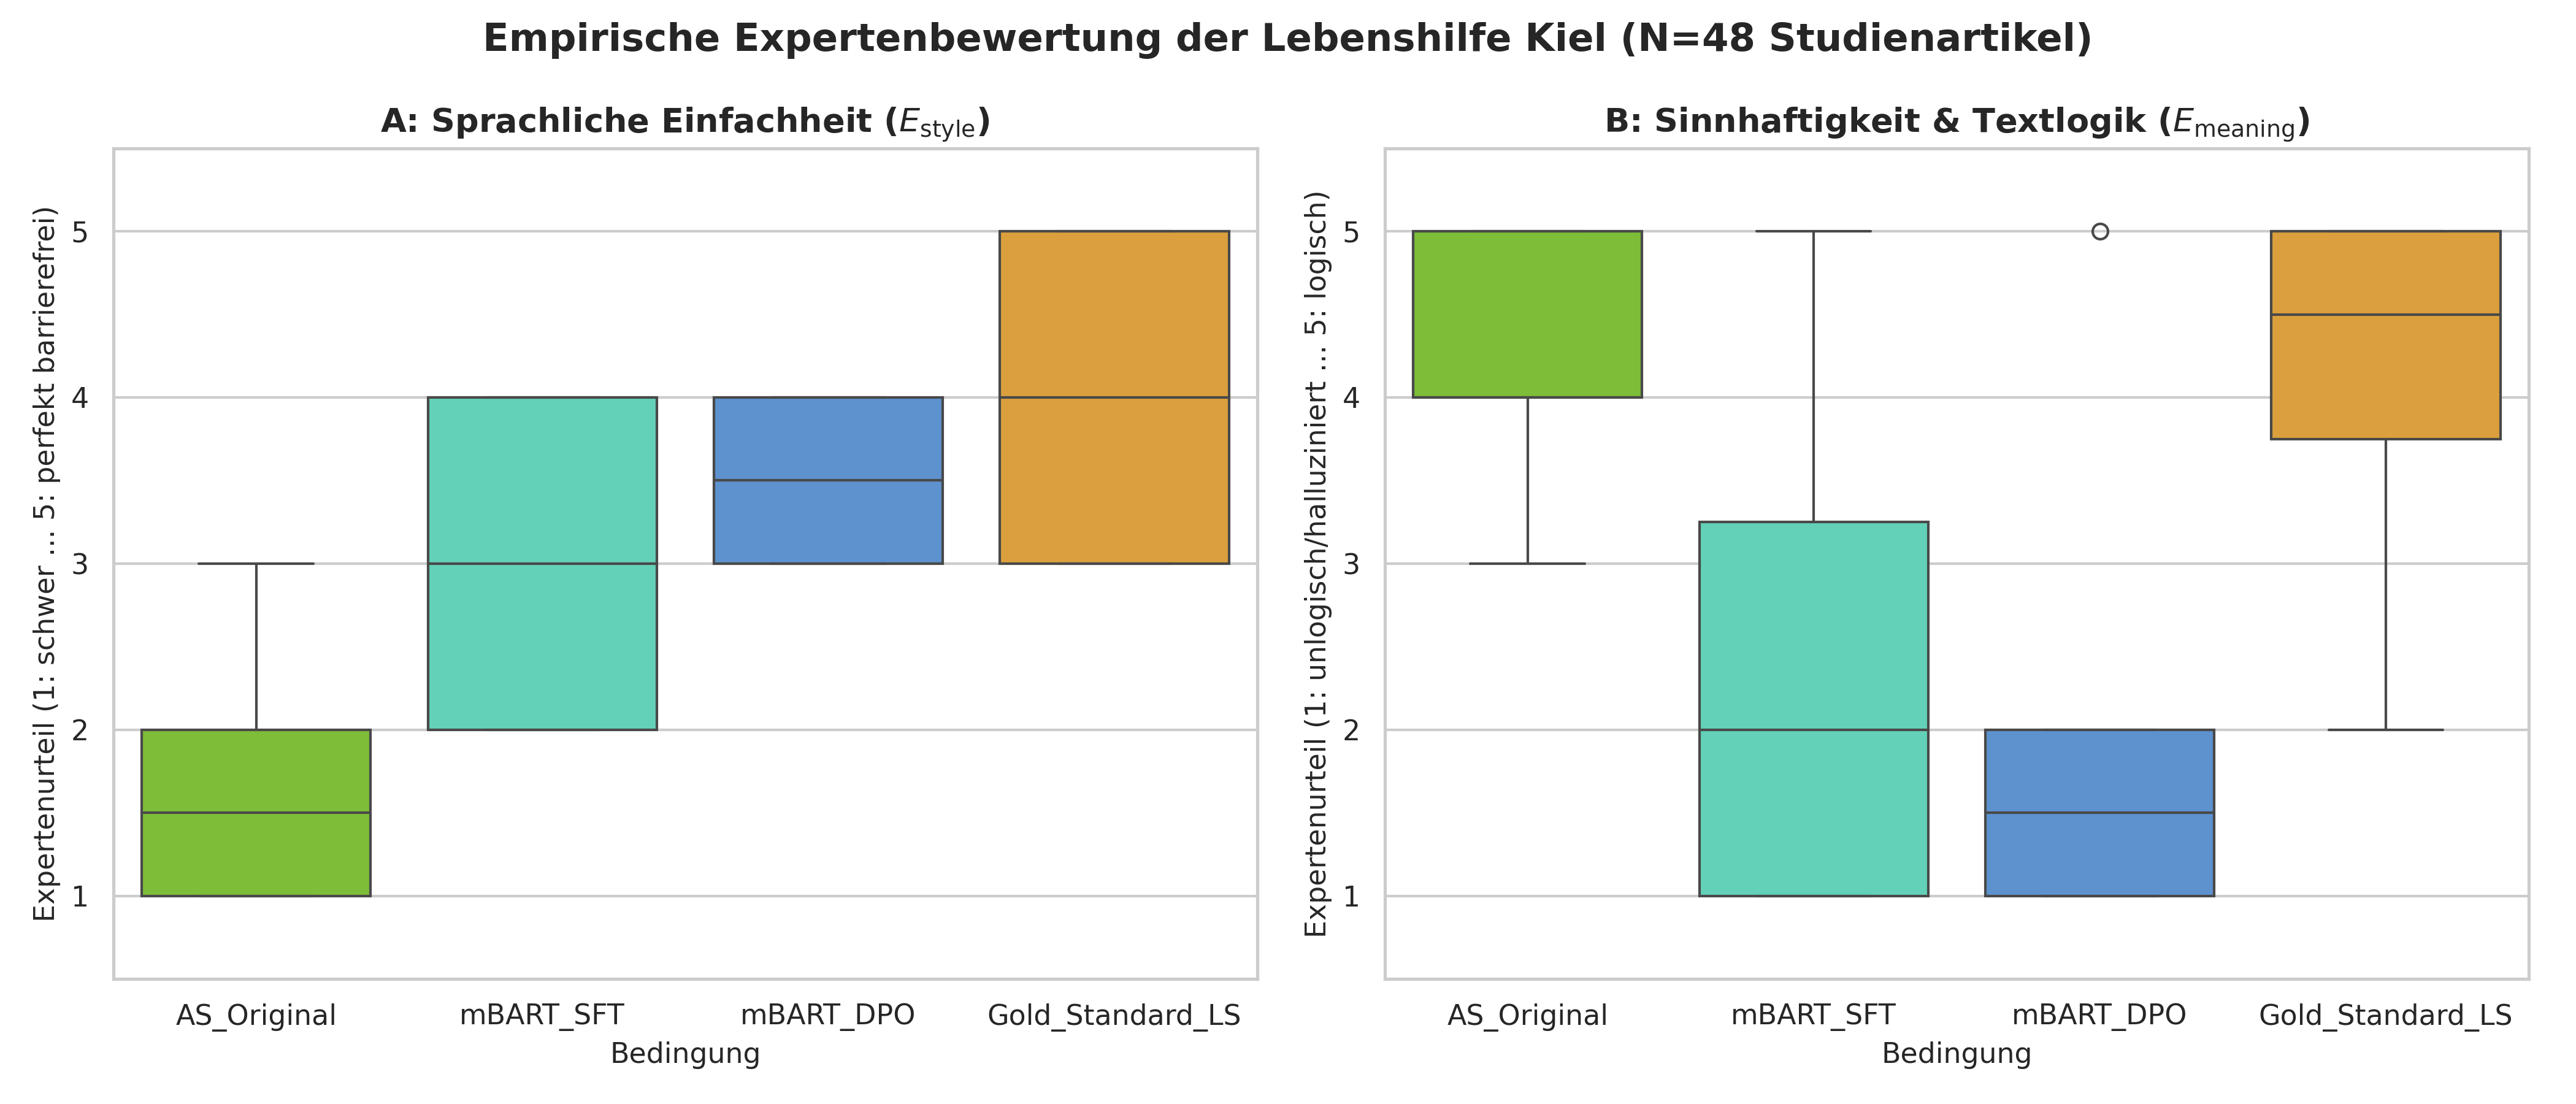
\includegraphics[width=0.95\textwidth]{images/expert_eval_boxplots_dual.png}
    \caption{Notenverteilung der Expertenbewertung über die vier Hauptbedingungen: (A) Sprachliche Einfachheit $E_{\text{style}}$ (1 = Alltagssprache bis 5 = sehr einfache Leichte Sprache) und (B) Sinnhaftigkeit und Textlogik $E_{\text{meaning}}$ (1 = unlogisch/Fehler bis 5 = klar verständlich).}
    \label{fig:expert_eval_boxplots_dual}
\end{figure}

\paragraph{Validierung der Metrik und Ergebnisse des Modellvergleichs:}
Die Auswertung der 50 Expertenbewertungen liefert folgende zentrale Erkenntnisse:
\begin{itemize}
    \item \textbf{Paarweise Rangübereinstimmung über 1.225 Textpaare:} Über die $\binom{50}{2} = 1.225$ kombinatorischen Paare erzielte der BiLSTM-MixUp-Regressor bei allen 959 eindeutig entschiedenen Paaren eine \textbf{Übereinstimmungsrate von 79{,}14\,\%} (759 passende vs. 200 abweichende Entscheidungen). Werden auch die 265 Texte einbezogen, die vom Experten identisch benotet wurden, liegt die Rangtreue bei 61{,}96\,\%.
    \item \textbf{Korrelation mit der Expertenbewertung (Einfachheit):} Der neuronale Regressor $R_{\text{style}}$ korreliert deutlich positiv mit dem Urteil der Fachperson ($\text{Spearman } \rho = 0{,}6750, \text{Pearson } r = 0{,}7864, p = 7{,}61 \times 10^{-8}$) und bildet die wahrgenommene Einfachheit präzise ab. Klassische Formeln wie der Flesch Reading Ease ($\rho = 0{,}5696$) oder der LIX-Index ($\rho = -0{,}5434$) weisen zwar ebenfalls eine moderate Korrelation auf, dies liegt jedoch primär daran, dass echte Leichte Sprache extrem kurze Sätze nutzt und diese rein längenbasierten Teilmengen somit zwangsläufig mitbedient (Teilmengen-Hypothese, vgl. Abschnitt~\ref{sec:klassifikator_laengen_ablation}). Wie die Analysen in Abschnitt~\ref{sec:klassifikator_laengen_ablation} zeigen, besitzen traditionelle Formeln für die Bewertung generierter Texte wenig eigenständige Aussagekraft, da sie gegenüber grammatikalischen Regelverletzungen (wie Passiv oder Konjunktiv) blind sind oder diese fälschlicherweise belohnen.
    \item \textbf{Modellentwicklung und Bestätigung der Pipeline (Abbildung~\ref{fig:expert_eval_boxplots_dual}A):} Die Verteilung der Expertennoten zeigt eine klare und kontinuierliche Steigerung der sprachlichen Einfachheit über die Modellierungsstufen: Ausgehend von den schweren Ausgangstexten der Alltagssprache ($E_{\text{style}} = 1{,}58$) bildet das SFT-Basismodell mit einer mittleren Note von $3{,}00$ das solide sprachliche Fundament. Durch die anschließende Präferenzoptimierung (DPO) wird dieses Signal über die Belohnungsmetrik nochmals gezielt verstärkt, sodass das DPO-Modell eine Einfachheit von $3{,}50$ erreicht und sich dem menschlichen Goldstandard ($3{,}92$) deutlich annähert. Dieses Ergebnis bestätigt exakt die quantitativen linguistischen Analysen aus Abschnitt~\ref{sec:dpo_rule_adherence}: Bereits das SFT-Training sorgt für eine deutliche Entflechtung und Vereinfachung gegenüber der Alltagssprache, während DPO die Regeleinhaltung und das Signal für einfache Satzstrukturen nochmals konsequent nachschärft.
    \item \textbf{Domänendifferenzierung des Goldstandards \& Trainingsbasis:} Bei der differenzierten Betrachtung der menschlichen Referenztexte (Tabelle~\ref{tab:expert_eval_results_master}) fällt auf, dass der Experte die In-Domain-Referenzen aus den Web-Quellen mit $E_{\text{style}} = 3{,}71 \pm 0{,}95$ spürbar schwächer bewertet hat als die Out-of-Domain-Texte der Lebenshilfe Kiel ($E_{\text{style}} = 4{,}20 \pm 0{,}84$). Bemerkenswert ist hierbei, dass die Bewertungen der generativen Modelle ($E_{\text{style}} = 3{,}50$ bei DPO bzw. $3{,}00$ bei SFT) deutlich näher an diesem In-Domain-Niveau der Web-Quellen liegen. Dies spiegelt wider, auf welcher Datenbasis die Modelle primär trainiert wurden: Da der Trainingsdatensatz überwiegend aus den frei zugänglichen Web-Quellen besteht, bildet das Modell naturgemäß genau den Sprach- und Qualitätsstandard dieser Web-Texte ab, während die professionell geprüften Lebenshilfe-Texte ein nochmals höheres Sprachniveau markieren.
    \item \textbf{Inhaltliche Fehler \& Textlogik (Abbildung~\ref{fig:expert_eval_boxplots_dual}B):} Während menschliche Gold-Texte ($4{,}17 \pm 1{,}03$) und Originaltexte ($4{,}25 \pm 0{,}75$) hohe Logiknoten erhalten, zeigen die maschinellen Modelle deutliche inhaltliche Schwächen (Halluzinationen in 58{,}3\,\% der Fälle bei SFT und 66{,}7\,\% bei DPO). Positiv ist, dass DPO Passivformen vollständig vermeidet ($0$ Fälle bei DPO vs. $4$ bei SFT und $9$ bei AS) und Worttrennungen mit Bindestrich konsequenter vornimmt. Die Ergebnisse verdeutlichen, dass eine rein formale Stiloptimierung künftig mit gezielten Prüfungen der inhaltlichen Richtigkeit kombiniert werden muss.
\end{itemize}
